\documentclass{ximera}
%\usepackage{sagetex}
%% handout
%% space
%% newpage
%% numbers
%% nooutcomes

%%% You can put user macros here
%% However, you cannot make new environments

\graphicspath{{./}{module1Activity/}{module2Activity/}{module3Activity/}}

\usepackage{sagetex}
\usepackage{tikz}
\usepackage{hyperref}
\usepackage{tkz-euclide}
\usetkzobj{all}
\pgfplotsset{compat=1.7} % prevents compile error.

\tikzstyle geometryDiagrams=[ultra thick,color=blue!50!black]
 %% we can turn off input when making a master document

\outcome{Understand the different sets of numbers along with the properties of these sets.}
\author{Darryl Chamberlain Jr.}
 
\title{Subgroups of Complex Numbers}

\begin{document}
\begin{abstract}
Identify the subgroup of Complex numbers a number belongs to. 
\end{abstract}
\maketitle

\href{https://cnx.org/contents/mwjClAV_@8.1:Sqk1HAGf@9/Complex-Numbers}{Link to section in textbook}

%%%%%%%%%%%%%%%%%%%%%
%%%  Objective 2  %%%
%%%%%%%%%%%%%%%%%%%%%

Now, watch \href{https://mediasite.video.ufl.edu/Mediasite/Play/8fae3825474042a297038c5d2385c4f51d}{this video} to review the different sets of Complex numbers. First, try to define the following subgroups of the Complex Numbers. You should include examples for each (you may even want to take a sneak peak at the problems at the bottom of the page and use some of these as examples!) and descriptions of how to tell what the smallest set the number belongs to. 

\begin{itemize}
\item Nonreal Complex:
\item Pure Imaginary:
\item Not a Complex Number: 
\end{itemize}

The Real Numbers are just a part of the Complex Numbers, so we still have the subgroups from Objective 1. Now we will look at how all of these subgroups are related. 

\begin{question}
Like before, we will visualize the groups in a chart. An empty chart is provided below. Fill in the subgroups and try to classify the following numbers: 

$$ -\frac{21}{7}+i, -\frac{7}{21}, \frac{21}{7}, \frac{\pi}{4}, \frac{4}{\pi}i, \frac{0}{\pi}, \frac{\pi}{0}i, -\sqrt{4}, \sqrt{-4}, \sqrt{21}, \sqrt{-21} $$

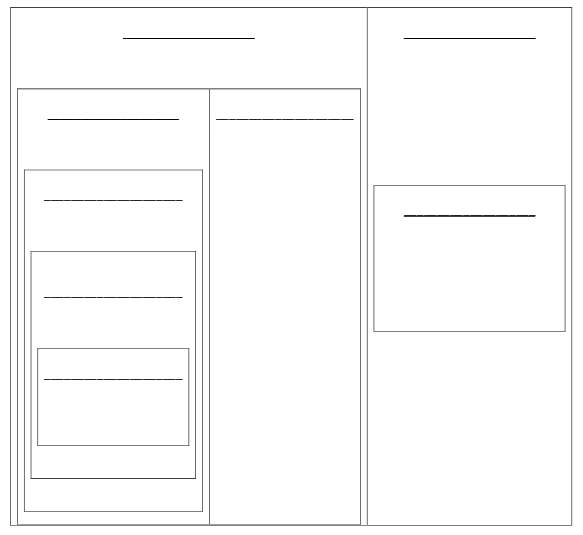
\includegraphics{complexNumbersChart.png}

\textbf{Smallest subgroup the number belongs to:} 

Natural: $\answer{\frac{21}{7}}$

Whole: $\answer{\frac{0}{\pi}}$

Integer: $\answer{-\sqrt{4}}$

Rational: $\answer{-\frac{7}{21}}$

Irrational: $\answer{\frac{\pi}{4}}$, $\answer{\sqrt{21}}$

Pure Imaginary: $\answer{\frac{4}{\pi}i}$, $\answer{\sqrt{-4}}$, $\answer{\sqrt{-21}}$

Nonreal Complex: $\answer{-\frac{21}{7} + i}$

Not a Complex Number: $\answer{\frac{\pi}{0}i}$

\end{question}

\textbf{Like Objective 1, remember to reduce first, then decide the smallest subgroup the number belongs to!}

\textbf{Note: This part of the homework will change each time you clikc ``Another". You can keep clicking ``Another" to practice seeing these more difficult numbers to classify.}

\begin{sagesilent}
# THIS code generates random Complex number. Options:
    # Rational
    # Irrational
    # Nonreal Complex
    # Pure Imaginary
    # Not a Complex number

# Structure of question:
    #  \frac{\sage{numerator}}{\sage{denominator}} + \sage{complexPart}

def generateRational():
    numerator = (ZZ.random_element(15)+2)*(-1)**(ZZ.random_element(2))
    denominator = ZZ.random_element(15)+2
    i = var('i')
    complexPart = (ZZ.random_element(15)+2)*i**2
    displayProblem = [numerator, denominator, complexPart]
    return displayProblem

def generateIrrational():
    numerator = (ZZ.random_element(2, 15))*(-1)**(ZZ.random_element(2))
    denominator = (ZZ.random_element(15)+2)*pi
    i = var('i')
    complexPart = (ZZ.random_element(15)+2)*i**2
    displayProblem = [numerator, denominator, complexPart]
    return displayProblem

def generateNonRealComplex():
    numerator = (ZZ.random_element(15)+2)*(-1)**(ZZ.random_element(2))
    denominator = (ZZ.random_element(15)+2)*pi
    i = var('i')
    complexPart = (ZZ.random_element(15)+2)*i
    displayProblem = [numerator, denominator, complexPart]
    return displayProblem

def generatePureImaginary():
    numerator = 0
    denominator = (ZZ.random_element(15)+2)*pi
    i = var('i')
    complexPart = (ZZ.random_element(15)+2)*i
    displayProblem = [numerator, denominator, complexPart]
    return displayProblem

def generateNotComplex():
    numerator = pi*(ZZ.random_element(15)+2)*(-1)**(ZZ.random_element(2))
    denominator = 0
    i = var('i')
    complexPart = (ZZ.random_element(15)+2)*i
    displayProblem = [numerator, denominator, complexPart]
    return displayProblem

def generateDisplay(answer):
    if answer == "Rational":
        numerator, denominator, complexPart = generateRational()
    elif answer == "Irrational":
        numerator, denominator, complexPart = generateIrrational()
    elif answer == "NonrealComplex":
        numerator, denominator, complexPart = generateNonRealComplex()
    elif answer == "PureImaginary":
        numerator, denominator, complexPart = generatePureImaginary()
    elif answer == "NotComplexNumber":
        numerator, denominator, complexPart = generateNotComplex()
    else:
        numerator, denominator, complexPart = [0, 0, 0]
        print "\n\n\n Something went wrong choosing how to display the problem. \n\n\n\n"
    return [numerator, denominator, complexPart]

def assignSetValue(set):
    if set == "Rational":
        value = 0
    elif set == "Irrational":
        value = 1 
    elif set == "NonrealComplex":
        value = 2
    elif set == "PureImaginary":
        value = 3
    elif set == "NotComplexNumber":
        value = 4
    else:
        value = 5
        print "Something went wrong when assigning the set a value. Please look into this."
    return value

############# END OF DEFINITIONS ###############

listOptions = ["Rational", "Irrational", "NonrealComplex", "PureImaginary", "NotComplexNumber"]

########## QUESTION 4 #############
set4 = sample(listOptions, 1)[0]
answer4 = assignSetValue(set4)
numerator4, denominator4, complexPart4 = generateDisplay(set4)

########## QUESTION 5 #############
set5 = sample(listOptions, 1)[0]
answer5 = assignSetValue(set5)
numerator5, denominator5, complexPart5 = generateDisplay(set5)

########## QUESTION 6 #############
set6 = sample(listOptions, 1)[0]
answer6 = assignSetValue(set6)
numerator6, denominator6, complexPart6 = generateDisplay(set6)
\end{sagesilent}

\begin{question}
Which of the following is the \textbf{smallest} set of Complex numbers that $\frac{\sage{numerator4}}{\sage{denominator4}} + \sage{complexPart4} $ belongs to?

\textit{To work around current Xronos issues, input the corresponding number for the correct set. \\
Rational - 0 \\
Irrational - 1 \\
Nonreal Complex - 2 \\
Pure Imaginary - 3 \\
Not a Complex Number - 4 
}

$\answer{\sage{answer4}}$

\end{question}

\begin{question}
Which of the following is the \textbf{smallest} set of Complex numbers that $\frac{\sage{numerator5}}{\sage{denominator5}} + \sage{complexPart5} $ belongs to?
	
\textit{To work around current Xronos issues, input the corresponding number for the correct set. \\
Rational - 0 \\
Irrational - 1 \\
Nonreal Complex - 2 \\
Pure Imaginary - 3 \\
Not a Complex Number - 4 
}
	
$\answer{\sage{answer5}}$
	
\end{question}

\begin{question}
Which of the following is the \textbf{smallest} set of Complex numbers that $\frac{\sage{numerator6}}{\sage{denominator6}} + \sage{complexPart6} $ belongs to?
	
\textit{To work around current Xronos issues, input the corresponding number for the correct set. \\
Rational - 0 \\
Irrational - 1 \\
Nonreal Complex - 2 \\
Pure Imaginary - 3 \\
Not a Complex Number - 4 
}
	
$\answer{\sage{answer6}}$
	
\end{question}

\end{document}
